\documentclass[SDSUThesis.tex]{subfiles} 
\begin{document}

% All about the SDLC Analytic Engine
\section{SDLC ANALYTIC ENGINE}
\label{sec:SDLC-AE}

    In order for an SDO to properly track the elements of CRI, a data storage 
    system should be available to store the appropriate data.  A consistent 
    storage system should help to avoid the problem of inaccurate
    data caused by numerous manipulations of the existing data 
    \cite{Olson2003}. Plus, if the system
    is implemented correctly by allowing limited changes to existing data, 
    it will be able to alleviate
    some of the dishonesty that is currently present in software projects 
    \cite{Rost2011}. This storage system will be named the SDLC Analytic 
    Engine (SDLC-AE). \nomenclature{SDLC-AE}{SDLC Analytic Engine}
    
    \begin{figure}[hbt]
        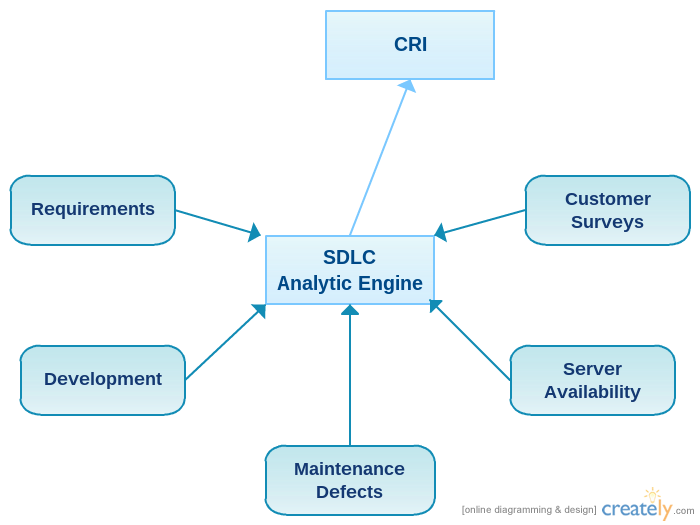
\includegraphics[scale=.75]{images/sdlcae.png}
        \caption{SDLC ANALYTIC ENGINE}
        \label{fig:sdlc-ae}
    \end{figure}
    
    
    Once all the SDLC data is collected into a single place, there are 
    many possible applications.  Software analytics
    will be much easier to create and gamification will be much more easily attainable.  
    CRI is just one possible application of the SDLC-AE.  Figure \ref{fig:sdlc-ae} 
    provides an overview of 
    the data that could potentially be stored in the SDLC-AE as it relates to CRI. The
    SDLC-AE does not specify how the data is entered, just how the data is stored.
    
    \subsection{DATABASE STRUCTURE}
        All the data necessary to compute CRI needs to be stored in a database.  This section will 
        lay out the structure of tables and relationships necessary to the store all the data
        within a relational database.  The SQL\footnote{Structured Query Language (SQL) is 
        a programming language designed for managing data in relational database 
        management system.\nomenclature{SQL}{Structured Query Language}} 
        is written for an Oracle
        database, but the scripts can be modified to work with other databases
        such as: PostgreSQL, SQL Server, or MySQL.  
        
        \subsubsection{TABLES FOR RAW CRI DATA}
        
            The first set of tables that need to be created are tables
            to store the raw data that is collected.  These tables
            will match up with the necessary data for each of the 5 elements
            of CRI.  Figure \ref{fig:raw} provides a visual description
            of the tables that are needed.  The tables have no relationship
            with each other since they are raw data.  The primary goal of
            these tables is to store the raw data in a single location. The
            5 table names are:
            \begin{enumerate}
                \item QUALITY\_RAW
                \item AVAILABILITY\_RAW
                \item SATISFACTION\_RAW
                \item SCHEDULE\_RAW
                \item REQUIREMENTS\_RAW
            \end{enumerate}
            Notice these table names match with the 5 elements of CRI.
        
           \begin{figure}[htb]
                \centering
                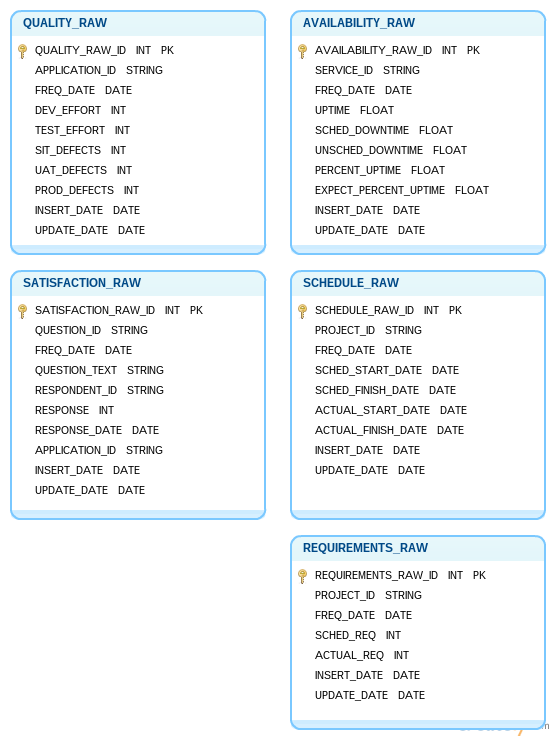
\includegraphics[scale=.52]{images/raw_tables.png}
                \caption{TABLES FOR RAW CRI DATA}
                \label{fig:raw}
            \end{figure}
            
            Appendix \ref{src:rawSQL} provides the necessary SQL statements to create the 
            database tables for storing the raw CRI data.  
            
        \subsubsection{INTERMEDIATE SCORE TABLES FOR CRI}
            The next set of tables that need to be created are for the 
            intermediate level element scores.  These tables hold the
            element scores at the application\_id, service\_id, and project\_id
            level.  Figure \ref{fig:score_tables} provides a visual overview
            of the necessary tables.  Furthermore, these tables also lack
            relationships between one another because at this point, all the
            element scores are still being treated independently.  The five
            table names are:
            
            \begin{enumerate}
                \item QUALITY\_SCORE
                \item AVAILABILITY\_SCORE
                \item SATISFACTION\_SCORE
                \item SCHEDULE\_SCORE
                \item REQUIREMENTS\_SCORE
            \end{enumerate}
            Again, these table names match very closely with the 5 elements of CRI.
        
           \begin{figure}[htb]
                \centering
                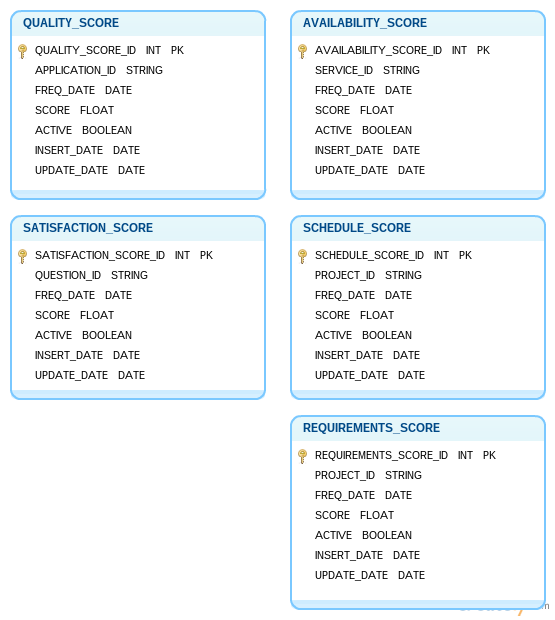
\includegraphics[scale=.52]{images/score_tables.png}
                \caption{TABLES FOR INTERMEDIATE CRI SCORES}
                \label{fig:score_tables}
            \end{figure}%
            
            Appendix \ref{src:scoreSQL} provides the necessary SQL statements to create the 
            database tables for storing the intermediate CRI scores.
        
        \subsubsection{FINAL SCORE TABLES FOR CRI}
            The final set of tables consists of only two tables.  
            \begin{enumerate}
                \item ELEMENT
                \item CRI\_SCORE
            \end{enumerate}
            The first
            table is the ELEMENT table.  It simply stores the CRI element 
            (Quality, Availability,Satisfaction,Schedule,Requirements,Overall) and 
            optional description. The second table is the CRI\_SCORE table.  
            It stores all the final element scores and the final overall CRI
            score.  It is related to the ELEMENT table.  Figure 
            \ref{fig:final_score_tables} provides a visual representation of the 
            relationship between the 2 tables. 
            
           \begin{figure}[hbt]
                \centering
                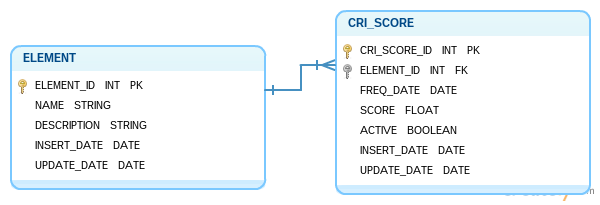
\includegraphics[scale=.52]{images/final_score_tables.png}
                \caption{TABLES FOR FINAL CRI SCORES}
                \label{fig:final_score_tables}
            \end{figure}
            
            
            Appendix \ref{src:overallscoreSQL} provides the necessary SQL 
            statements to create the 
            database tables for storing the final scores for each element and the final 
            overall CRI scores for each time frequency.

\end{document}







